\section{Расширение изначально однородно заряженного шара}

\textit{Первый метод}. 

Рассмотрим эту задачу с точки зрения симметрии. Во-первых, понятно, что в системе отсутствует магнитное поле. Во-вторых, плотность заряда $\rho$ и поле скоростей $\vec{v}$ зависят только от расстояния до центра шара. Также скорость имеет только одну компоненту $v_r$, также как и электрическое поле $E_r$.
 
Выберем внутри шара радиуса $R$ заряд которой равен $Q$ сферу радиуса $r_0$. Такая сфера ограничивает заряд:
\[
	q = \frac{r_0^3}{R^3} Q
\]

Найдём как движется точка на поверхности такой сферы. Уравнение движения:
\[
	\frac{d^2 r}{dt^2} = \alpha E_r = \alpha  k \frac{q}{r^2}
\]
\[
	\frac{v_r^2}{2} - \frac{v_{0r}^2}{2} = \alpha k q \left(- \frac{1}{r} + \frac{1}{r_0}\right)
\]
\[
	v_r = \sqrt{v_{0r}^2 + \frac{2\alpha kq}{r_0} - \frac{2\alpha k q}{r}} = \sqrt{a - \frac{b}{r}}
\]
\[
	\int\limits_{r_0}^{r} 
	\frac{\sqrt{r} dr}{\sqrt{ar - b}}
	=
	t - t_0
\]
\[
	\frac{b}{a^{3/2}} 
	\left.
	\left(\sqrt{\frac{ar}{b}} \sqrt{\frac{ar}{b}-1} + 
	\ln \left|\sqrt{\frac{ar}{b} - 1} + \sqrt{\frac{ar}{b}}\right|\right) 
	\right|_{r_0}^{r}
	= t - t_0
\]
В случае если $v_{r}(0) = 0$, получаем:
\[
	b = 2\alpha k q
\]
\[
	a = \frac{2\alpha kq}{r_0}
\]
\[
	\frac{r_0^{3/2}}{(2\alpha k q)^{1/2}} 
	\left(\sqrt{\frac{r}{r_0}} \sqrt{\frac{r}{r_0}-1} + 
	\ln \left|\sqrt{\frac{r}{r_0} - 1} + \sqrt{\frac{r}{r_0}}\right|\right)
	= t
\]
\[
	\left(\sqrt{\frac{r}{r_0}} \sqrt{\frac{r}{r_0}-1} + 
	\ln \left|\sqrt{\frac{r}{r_0} - 1} + \sqrt{\frac{r}{r_0}}\right|\right)
	= \sqrt{
		\frac{2\alpha k Q}{R^{3}} } t = f\left(\frac{r}{r_0}\right)
\]
На рисунке приведена зависимость $r(t)$, для различных значений $r_0$.
\begin{figure}[h!]
	\centering
	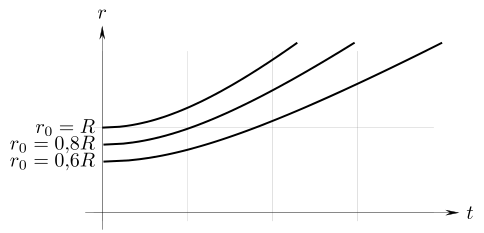
\includegraphics{images/png/sphere1.png}
\end{figure}
\\
Плотность зарядов можно найти, определяя для каждого из слоёв, между которыми находится заряд $dq$, толщина между слоями $dr_0$, в момент времени $t$ соответствующее расстояние между слоями:
$dr$:
\[
\rho = \frac{1}{4\pi r^2} \frac{dq}{dr},
\]
где $dr$ определяется $dr_0$, а $dt = 0$. В результате:
\[
	f'\left(\frac{r}{r_0}\right) \frac{dr}{r_0} = f'\left(\frac{r}{r_0}\right) \frac{r dr_0}{r_0^2} 
\]
\[
	\frac{dr}{r} = \frac{dr_0}{r_0}
\]
\[
	\rho = \frac{Q}{4\pi R^3/3} \left(\frac{r_0}{r}\right)^3 = \rho_0 \left(f^{-1}\left(\sqrt{
		\frac{2\alpha k Q}{R^{3}} } t\right)\right)^{-3}
\]
То есть $\rho$ зависит только от времени и не зависит от расстояния, что означает, что шар всегда однороден.